% !TeX encoding 	= utf8
% !TeX program 		= pdflatex
% !TeX spellcheck 	= de-DE
% !BIB = biber

\RequirePackage[l2tabu, orthodox]{nag}			% Sucht nach Fehlern und gibt Warnung aus (.log)

% ---------------------------
% Dokumentklasse
% ---------------------------
% Mögliche Optionen:
%	- parskip = half; full, none
% 	- Schriftgröße (11pt [default], 12pt)
%	- Papiergröße (a4paper [default], a5paper)
%	- zweiseitig (twoside, oneside [default])	 
% ---------------------------

\documentclass[
    12pt,										% Schriftgröße
    a4paper,									% Papiergröße
    parskip 	= half,							% Definiert Absätze
    listof		= totoc,						% Abb.- und Tab.-verzeichnis
    bibliography= totoc,						% Quellenverzeichnis
%    twoside,									% Zweiseitiger Druck
    version 	= last,							% Version
%    heading		= small,
	numbers		= noenddot,
]{article}										% Komascript (vorzugsweise zu verwenden)

% ---------------------------
% Einbinden von Packages
% ---------------------------
% ---------------------------
% Wichtiger Hinweis für die Kodierung:
% 	Inputenc gibt die Kodierung des Dokoments an,
% 	die muss mit der Kodierung der Datei übereinstimmen.
% 	
%   Mögliche Einstellungen:
%	Editor		|	inputenc
%	------------|------------
%	UTF-8		|	utf8			(vorzugsweise verwenden)
%	ISO-8859-1	|	ansinew
%	windows-1252|	ansinew
%	Apple		|	applemac		(von mir nicht geprüft)
%	Linux		| 	latin1, utf8
% ---------------------------

% --- Kodierung, Sprache ---
\usepackage[utf8]{inputenc}						% Kodierung des Dokuments
\usepackage[T1]{fontenc}						% Schriftzeichen, Umlaute, Silbentrennung
\usepackage[ngerman]{babel}						% Neue deutsche Rechtschreibung
\usepackage[printonlyused]{acronym}				%b Abkürzungsverzeichnis

% --- Schrift ---
\usepackage{lmodern}							% Moderne Schriftart
\usepackage{microtype}							% Randausgleich und Neuberechnung der Lücken

% ---------------------------
% Fakulative Packages
% ---------------------------
% Zum Aktivieren Kommentar entfernen
% 
%		---WICHTIG---
% Reihenfolge von einigen Pakete muss beachtet werden, 
% da es ansonsten zu "Option clash" kommen kann!
% ---------------------------

% --- Hacks ---
\usepackage{scrhack}							% Hacks für setspaces, float, hyperref und listings


% --- Tabellen ---
\usepackage{tabularx}							% Verwendung der Tabularx-Umgebung für Tabellen
\usepackage{booktabs}							% Übersichtlichere Darstellung von Tabellen
\usepackage{multirow}							% Zusammenfassen von Tabellenreihen (vertical)


% --- Grafiken ---
\usepackage{graphicx} 							% Einbinden von Bildern
%\usepackage{float}								% U.a neue Option H für figure und table


% --- Formatierungen und Design ---
\usepackage{setspace}							% Ein-, anderhalb- oder zweizeilig
\usepackage[%
	% --- Linienart ---							% Einstellung von Dicke und Breite
%	headtopline,								% durch name = Dicke:Breite
%	plainheadtopline,
	headsepline,
%	plainheadsepline,
%	footsepline,
	plainfootsepline,
%	footbotline,
%	plainfootbotline,
%	ilines,
	clines,
%	olines,
	automark,
%	autooneside = false,						% ignore optional argument in automark at oneside
]{scrlayer-scrpage}								% Kopf- und Fußzeile
\usepackage[
	top 	= 2.5cm,								% Seitenabstand oben
	right 	= 2.5cm,								% Seitenabstand recht			
	bottom 	= 2.5cm,								% Seitenabstand unten
	left	= 2.5cm,								% Seitenabstand links
	includeheadfoot,							% Zitate als Fußnote
	bindingoffset = 1cm							% Bindekorrektur								
]{geometry}
\usepackage[
	table,
	dvipsnames									% Vordefinierte Farben
]{xcolor}										% Farbige Darstellungen
%\usepackage{caption}							% Bilder- u. Tabellenbeschriftung
\usepackage{listings}


% --- Mathematik ---
%\usepackage{cancel} 							% Durchstreichen von Gleichungen
\usepackage{siunitx}							% Darstellung von Maßzahlen und Maßeinheiten
\usepackage[
	intlimits,  								% Grenzen Integral
	%leqno,     								% Nummerierung links
	%reqno,     								% Nummerierung rechts [default]
	%fleqn      								% Formel linksbündig mit festem Abstand
]{amsmath}										% Erweiterung des Mathemodus
\usepackage[
	all,
	warning,
%	error										% Kompilieren von pdfLaTeX kann abgebrochen werden
]{onlyamsmath}									% Anzeigen von Fehlern bei Verwendung von amsmath
%\usepackage[
%	fixamsmath,									% [default]
%	disallowspaces								% Fehlerbehebung
%]{mathtools}									% Erweitung zu amsmath


% --- PDF ---
%\usepackage{epstopdf}							% Konvertiert .eps zu .pdf on-the-fly (graphicx notwendig!)
%\usepackage{pdfpages}							% PDF Seiten einbinden


% --- Quellenangabe
\usepackage[autostyle]{csquotes}				% Anführungszeichen für deutsche Sprache und Quellenverzeichnis
\usepackage[%
	backend			= biber,					% bibtex oder biber [default]
	style			= numeric,    				% Literaturverzeichnisstil
	citestyle		= authortitle-icomp,		% Zitierstil
	sorting			= nty,						% Sortierung (Name, Titel, Jahr)
	natbib			= true,						% Kompatibilität mit Natbib-Bibliothek
	isbn			= false,					%
	url				= true,						%
	doi				= false,					%
	eprint			= false,					%
	block			= space,            		% kleiner horizontaler Platz zwischen den Feldern
	backrefstyle	= three+,       			% fasst Seiten zusammen, z.B. S. 2f, 6ff, 7-10
	date			= short,           			% Datumsformat
	bibwarn			= true,						%
	texencoding		= auto, 					% auto-detect the input encoding
	bibencoding		= auto 						% (auto (equal to tex), <encoding>)
]{biblatex}
%\usepackage[
%	square,
%	numbers
%]{natbib}										% Zitierstile (NUR für bibtex!)


% --- Zusatzpakete ---
\usepackage{blindtext}							% Ermöglichst Benutzung von Blindtext
\usepackage{tikz}
\usepackage{algorithm}							% Ermöglicht Erstellung von Algorithmen
\usepackage{algpseudocode}

% --- Verweise ---
\usepackage[hidelinks]{hyperref}				% Ermöglicht Verlinkungen [Immer als letztes!]


% ---------------------------
% Einstellungen von Optionen
% ---------------------------

% --- Macro importieren ---
%-------------------------------------
%-- Informationen für das Deckblatt --
%-------------------------------------
\newcommand{\titel}{\textbf{Studienarbeit}}
\newcommand{\thema}{Real World Integration}
\newcommand{\studiengang}{Informationstechnik}
\newcommand{\dhbw}{Dualen Hochschule Baden-Württemberg Mannheim}
\newcommand{\dlr}{Deutsches Zentrum für Luft- und Raumfahrt e. V.}
\newcommand{\jahrgang}{\textit{MA-TINF13ITIN}}

\newcommand{\praxis}{von hier bis da}
\newcommand{\betreuer}{Prof. Dr. Harald Kornmayer}
\newcommand{\abgabe}{abgabe ist irgendwann}

\newcommand{\autorA}{\textbf{Tobias Haase}}
\newcommand{\matrikelnrA}{4577806}
\newcommand{\autorB}{\textbf{Sven Durchholz}}
\newcommand{\matrikelnrB}{6002482}
\newcommand{\autorC}{\textbf{Phillipp Mevenkamp}}
\newcommand{\matrikelnrC}{9893674}
\newcommand{\autorD}{\textbf{Hendrik Abbenhaus}}
\newcommand{\matrikelnrD}{1234567}

%----------------------------------
%-- Vordefinierte Formatierungen --
%----------------------------------

%format: \setEquation{gleichung}{label for references}
\newcommand{\setEquation}[2]
{
	\begin{figure}[!htbp]
		\centering
		\begin{equation}
			#1
		\end{equation}
		\label{eq:#2}
	\end{figure}
}

%format: \setPicture{path}{description}{label for references}
\newcommand{\setPicture}[3]{
	\begin{figure}[!htbp]
		\centering
		\includegraphics[width=\textwidth]{#1}
		\caption{#2}
		\label{fig:#3}
	\end{figure}
}

%format: \setPicture{path}{width}{description}{label for references}
\newcommand{\setPictureWidth}[4]{
	\begin{figure}[!htbp]
		\centering
		\includegraphics[width=#2]{#1}
		\caption{#3}
		\label{fig:#4}
	\end{figure}
}

%format: \setPictureSourced{path}{width}{description}{label for references}{source}
\newcommand{\setPictureSourced}[5]{
	\begin{figure}[!htb]
		\centering
		\includegraphics[width=#2]{#1}
		\caption[#3]{#3\protect\footnotemark}
		\label{fig:#4}
	\end{figure}
	\footnotetext{Quelle: \citeauthor{#5}, \citetitle{#5}}
}

%format: \setTable{path}{description}{label for references}
\newcommand{\setTable}[3]{
	\begin{figure}[!htbp]
		\centering
		\input{#1}
		\caption{#2}
		\label{#3}
	\end{figure}
}

%format: \refPicture{label for references}
\newcommand{\refPicture}[1]{\figurename~\ref{fig:#1}}
\newcommand{\refTable}[1]{\tablename~\ref{tab:#1}}
\newcommand{\refChapter}[1]{Kapitel \ref{#1}}
\newcommand{\refEquation}[1]{Gleichung \ref{eq:#1}}


% ---------Schriftformatierungen------------------ 
\newcommand{\Name}[1]{\emph{#1}}
\newcommand{\Fachbegriff}[1]{\textbf{#1}} 
\newcommand{\Code}[1]{\texttt{#1}}
\newcommand{\Datei}[1]{\texttt{#1}}
\newcommand{\Datentyp}[1]{\textsf{#1}}

% ---------- Other -----------
\newcommand{\cpp}{C\texttt{++}}
\newcommand{\csh}{C\texttt{\#}}

% --- Paketeinstellungen ---
% --- Farben definieren ---
\definecolor{mygreen}{rgb}{0,0.6,0}
\definecolor{mygray}{rgb}{0.5,0.5,0.5}
\definecolor{mymauve}{rgb}{0.58,0,0.82}

% --- Formattierung Quellcode ---
% https://en.wikibooks.org/wiki/LaTeX/Source_Code_Listings
\lstset{ %
  backgroundcolor=\color{white},   % choose the background color; you must add \usepackage{color} or \usepackage{xcolor}
  basicstyle=\footnotesize,        % the size of the fonts that are used for the code
  breakatwhitespace=false,         % sets if automatic breaks should only happen at whitespace
  breaklines=true,                 % sets automatic line breaking
  captionpos=b,                    % sets the caption-position to bottom
  commentstyle=\color{mygreen},    % comment style
  deletekeywords={...},            % if you want to delete keywords from the given language
  escapeinside={\%*}{*)},          % if you want to add LaTeX within your code
  extendedchars=true,              % lets you use non-ASCII characters; for 8-bits encodings only, does not work with UTF-8
  frame=single,	                   % adds a frame around the code
  keepspaces=true,                 % keeps spaces in text, useful for keeping indentation of code (possibly needs columns=flexible)
  keywordstyle=\color{blue},       % keyword style
  otherkeywords={*,...},           % if you want to add more keywords to the set
  numbers=left,                    % where to put the line-numbers; possible values are (none, left, right)
  numbersep=5pt,                   % how far the line-numbers are from the code
  numberstyle=\tiny\color{mygray}, % the style that is used for the line-numbers
  rulecolor=\color{black},         % if not set, the frame-color may be changed on line-breaks within not-black text (e.g. comments (green here))
  showspaces=false,                % show spaces everywhere adding particular underscores; it overrides 'showstringspaces'
  showstringspaces=false,          % underline spaces within strings only
  showtabs=false,                  % show tabs within strings adding particular underscores
  stepnumber=2,                    % the step between two line-numbers. If it's 1, each line will be numbered
  stringstyle=\color{mymauve},     % string literal style
  tabsize=2,	                   % sets default tabsize to 2 spaces
  title=\lstname                   % show the filename of files included with \lstinputlisting; also try caption instead of title
}

% --- mathtools ---
%\mathtoolsset{showonlyrefs}					% Nummierung von Gleichungen nur, wenn diese einen Verweis besitzen

% --- siunitx ---
\sisetup{
%	mode = math, % text is printed using a math font
	detect-all,
	separate-uncertainty 	= true,				% Plus-Minus-Zeichen für Fehler
	exponent-product 		= \cdot,			% Malzeichen für Exponent
	number-unit-separator 	= \text{\,},		% Komma als Dezimalzeichen statt Punkt
	output-decimal-marker 	= {\text{,}},
	per-mode 				= fraction,			% Darstellung von Brüchen
}

% --- caption ---
%\captionsetup{}

% --- scrlayer-scrpage ---
%\pagestyle{scrheadings}
\clearpairofpagestyles							% Leeren von Kopf- und Fußzeile

%\ohead{\pagemark} 								% Kopfzeile außen: Seitenzahl
\ihead{\headmark} 								% Kopfzeile innen: chapter und section Titel
\cfoot[-~\pagemark~-]{-~\pagemark~-}			% Fußzeile mitte: Seitenzahl
%\setkomafont{pageheadfoot}{}					% Änderung von Kopf- und Fußzeile
%\setkomafont{pagenumber}{}
%\setkomafont{headsepline}{\color{red}}

% --- hyperref ---
\hypersetup{
	pdftitle 			= {Studienarbeit},		% Name des Dokuments
	pdfsubject 			= {Real World Integration},% Thema der Dokuments
	pdfauthor 			= {},				% Autor
%	pdfkeywords 		= {},
%	pdfcreator 			= {},
%	pdfproducer 		= {},
	pdftoolbar 			= true,
	pdfmenubar 			= false,
%	bookmarks 			= true,
	bookmarksopen 		= false,				% bookmarksopen ODER bookmarksopenlevel!
%	bookmarksopenlevel 	= section,
}

% --- biblatex ---
\DefineBibliographyStrings{german}{				% "Datum" für URL in Zitaten
	urlseen = {Besucht:}
}

% ---------------------------
%\KOMAoptions{
%	headlines	= 2								% Für mehrzeilige Überschriften
%	headinclude,								% Überschrift in Satzspiegel berücksichtigen
%	BCOR		= 1cm,							% Bindekorrektur
%	DIV			= calc							% Satzspiegel neuberechnen
%}

% ---------------------------
% Allgemeine Einstellungen
% ---------------------------

% --- Stil der Seitenzahlen ----
\pagenumbering{Roman}							% Möglichkeiten: arabic [default], Roman, Alpha, gobble (keine Nummerierung)

% --- Angabe des Speicherorts von Bildern ---
\graphicspath{{images/}}							% NUR in Verbindung mit graphicx!

% ---------------------------
% Beginn des Dokuments
% ---------------------------
\begin{document}

\begin{titlepage}
	\centering
	{\scshape\LARGE DHBW Mannheim \par}
	\vspace{1cm}
	{\scshape\Large Robotik Projekt\par}
	\vspace{1.5cm}
	{\huge\bfseries Vier Gewinnt auf einer LED-Matrix\par}
	\vspace{2cm}
	{\Large\itshape Sven Durchholz und Julian Kaping\par}
	\vspace{1cm}
	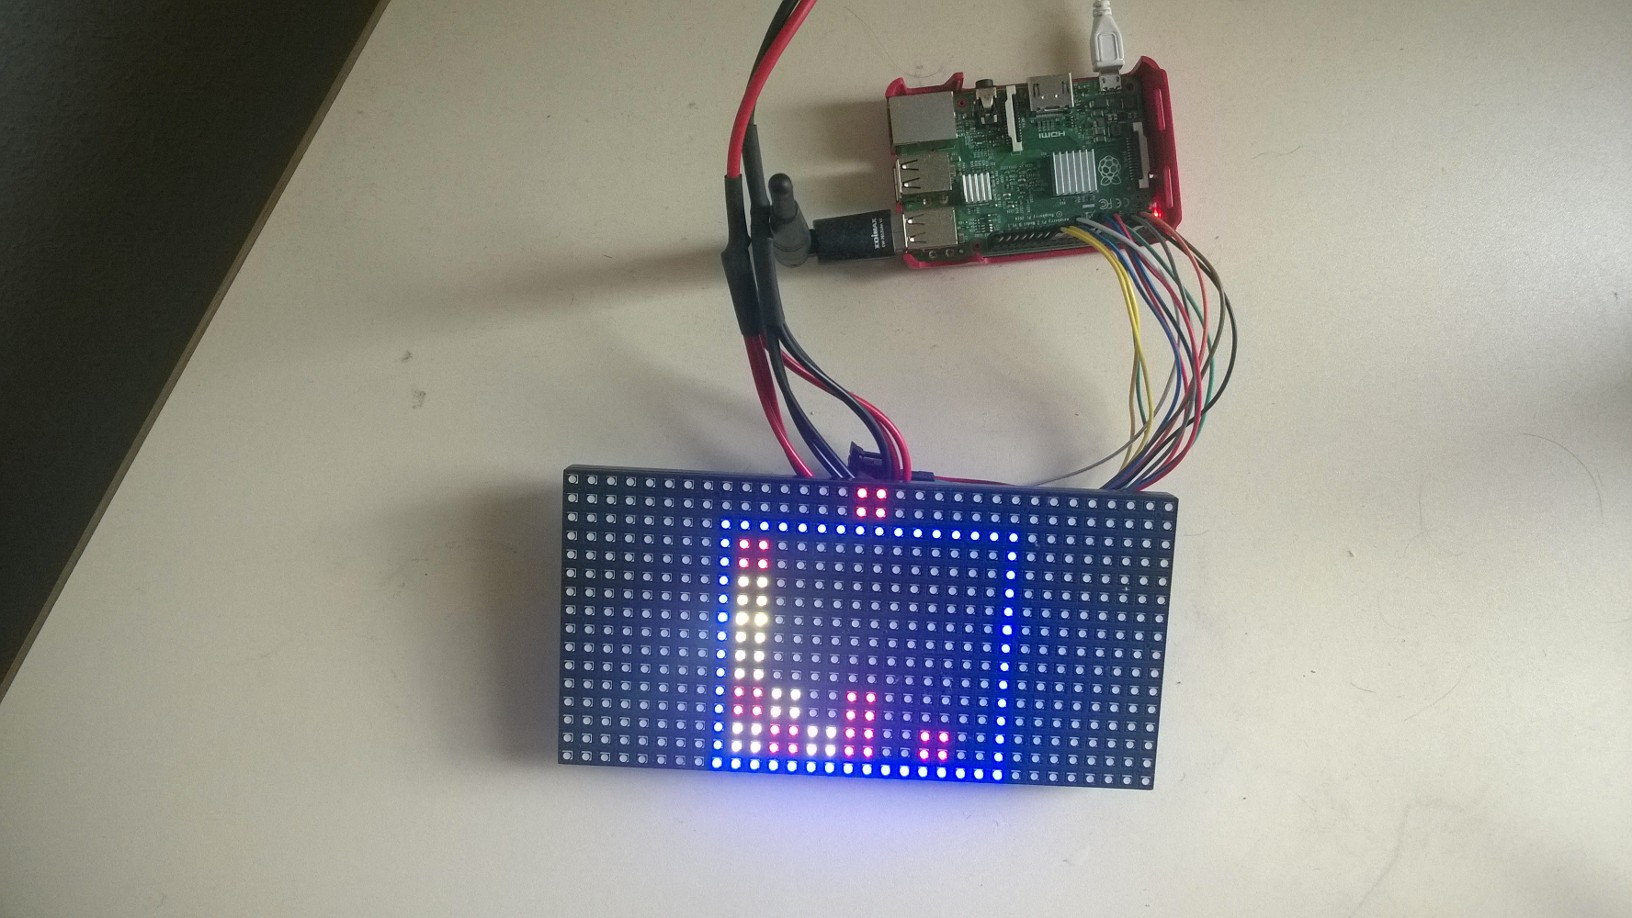
\includegraphics[width=0.9\textwidth]{inAction.jpg}\par\vspace{1cm}
	\vfill

% Bottom of the page
	{\large \today\par}
\end{titlepage}
	
	% ---------------------------
	% Kapitel und Abschnitte
	% ---------------------------
	\pagenumbering{arabic}
	\onehalfspacing
	
	
	\section{Einleitung}
Ziel der Arbeit im Rahmen der Vorlesung Robotik war es, das Spiel \glqq Vier Gewinnt\grqq ~auf einer LED-Matrix zu implementieren und eine Künstliche Intelligenz zu entwickeln, die es ermöglicht auch alleine das Spiel zu nutzen.

\section{Vier Gewinnt}
\label{sec:vierg}
Bei \glqq Vier Gewinnt\grqq ~handelt es sich um ein Spiel, bei dem zwei Spieler auf einem klassischerweise 6x7 Feld (6 Zeilen, 7 Spalten) versuchen über das jeweilige Setzen von Steinen eine Reihe von vier Steinen zu erzeugen. Die Vorraussetzungen dabei sind, dass der jeweilige Stein am unteren Ende der Spalte gesetzt wird und die Spieler stets nacheinander am Zuge sind.

\begin{figure}[!hbt]
	\centering
	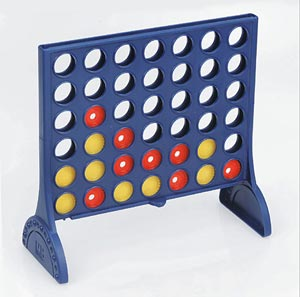
\includegraphics[scale=0.8]{4Gewinnt.jpeg}
	\caption{Ein klassisches Vier-Gewinnt-Spiel}
\end{figure}

Aus mathematischer Sicht ist \glqq Vier Gewinnt\grqq ~ein Spiel mit perfekter Information. Dies bedeutet, dass zu jedem Zeitpunkt alle vorhergehenden Züge bekannt sind. Diese perfekte Information sorgt dafür, dass das Spiel vollständig gelöst werden kann. Daraus kann abgeleitet werden, dass der Ausgang des Spiels für zwei perfekt spielende Gegner davon abhängig ist, in welche Spalte der erste Stein gesetzt worden ist: Wurde der erste Stein in die mittlere Spalte gesetzt, so gewinnt bei perfektem Spiel stets der erste Spieler. Beim Setzen in eine der Nachbarspalten, endet das Spiel unentschieden, sollte der erste Stein in eine der übrigen Spalten gesetzt werden, so gewinnt der zweite Spieler. 

\section{LED-Matrix und Darstellung des Spielfeldes}
\label{sec:ledm}
Um \glqq Vier Gewinnt\grqq ~auf einer LED-Matrix abbilden zu können müssen zwei wesentliche Eigenschaften von der Matrix erfüllt werden: Zunächst muss die Matrix eine Mindestgröße von 6x7 besitzen, zum anderen muss sie fähig sein mindestens zwei unterschiedliche Farben abzubilden.
Bei der Suche nach einer geeigneten Matrix hat sich herausgestellt, dass vor allem die zweite Eigenschaft ein Problem darstellt.
Es konnte dennoch eine geeignete Matrix gefunden werden:
Das \glqq Adafruit 16x32 RGB LED matrix panel\grqq.

\begin{figure}[!hbt]
	\centering
	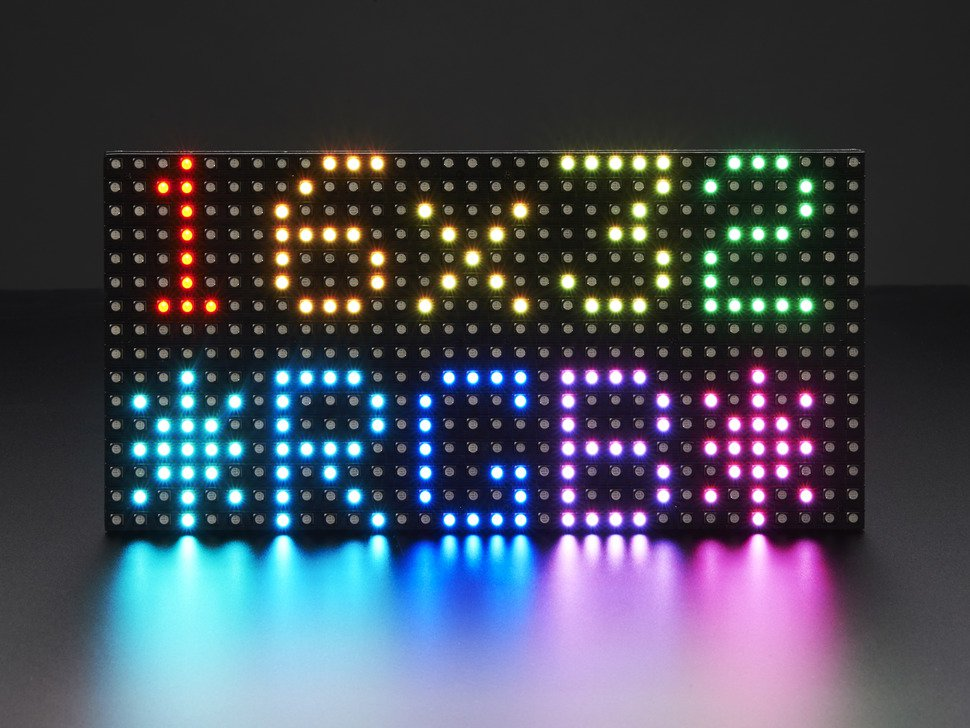
\includegraphics[scale=1]{RGBLEDMatrix.jpg}
	\caption{Verwendete LED-Matrix von Adafruit}
\end{figure}

Da die Matrix mit 16x32 deutlich über der Anforderung lag, wurde entschieden, dass auf der Matrix jeder Stein durch ein 2x2 Feld  dargestellt wird.
Das Feld würde somit eine Fläche von 12x14 einnehmen. Da somit immer noch genügend Platz vorhanden ist, und die Matrix mehr als zwei Farben anbietet, soll das Spielfeld durch einen Rand in einer anderen Farbe begrenzt werden.
Die somit ausgefüllte Fläche beträgt 14x16.
Zur besseren Visualisierung wurde zuletzt noch entschieden, über dem Spielfeld durch einen blinkenden Stein sowohl darzustellen, welcher Spieler aktuell am Zug ist, als auch in welche Spalte der nächste Stein aktuell gesetzt werden würde.
Insgesamt wird somit die Hälfte der Matrix genutzt, ein 16x16 Feld.
Aus ästhetischen Gründen wird daher das gesamte Feld in der Mitte der Matrix angezeigt.

\section{Ansteuerung der Matrix}
Zur Steuerung des Spielverlaufs ist ein Computer notwendig, welcher die Logik des 4 Gewinnt Spiels simulieren kann. Der Computer muss über 12 GPIO Pins zur Ansteuerung der LED-Matrix verfügen. Für diesen Zweck kommt ein \glqq Raspberry Pi 2 Model B\grqq{} zum Einsatz, welcher über 26 GPIOs Pins sowie weitere Pins für Masse und Stromversorgung verfügt.

\begin{figure}[!hbt]
	\centering
	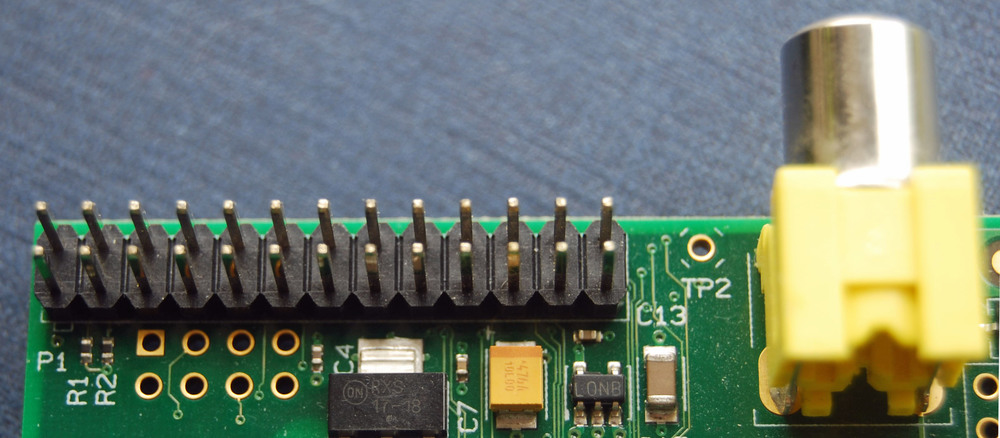
\includegraphics[scale=1]{gpio-pins}
	\caption{Nahaufnahme der Pins eines Raspberry Pis 2 Model B}
\end{figure}

Die GPIOs des Raspberry Pis werden mithilfe von mehreren Male/Female Jumpern mit der LED-Matrix verbunden. Um eine bessere Transportierbarkeit zu gewährleisten wird ein Aufsatz auf die GPIOs des Raspberry Pis verwendet. Die Verkabelung wird auf dem Aufsatz ausgeführt und dieser anschließend auf die GPIOs des Raspberry Pis gesteckt. Der Aufsatz ist abnehmbar und der Raspberry Pi somit unabhängig von der Verkabelung.

Für die Ansteuerung wird die Matrix ab der achten Zeile in zwei Hälften unterteilt. Beide Hälften können gleichzeitig angesteuert werden, um die Effizienz zu steigern. Um die darzustellende Farbe zu bestimmen sind je Hälfte 3 Pins notwendig welche die RGB-Werte einer LED darstellen. Durch unterschiedliche Kombinationen der auf den Pins anliegenden Werte können dabei bis zu 7 unterschiedliche Farben (+ dem Auszustand) auf den LEDs angezeigt werden. Weiter verfügt die Matrix über eine sogenannte \glqq clock \grqq{} mit der durch die einzelnen Spalten iteriert werden kann. Die \glqq clock \grqq{} wird dafür an einem GPIO des Raspberry Pis angeschlossen. Sobald ein Signal auf den Pin gelegt wird, wird die angesprochene LED um eine Spalte erhöht. Um die Zeile zu wählen werden 3 GPIO Pins angeschlossen. Diese stellen ein Binäres Signal zwischen 0 und 7 dar, welches die anzusprechende Zeile darstellt. Ein weiterer GPIO dient dabei als Signal um den Reihenwechsel zu initialisieren. Der verkabelte Aufbau kann in Abbildung \ref{verkabelung} betrachtet werden.

\begin{figure}[!hbt]
	\centering
	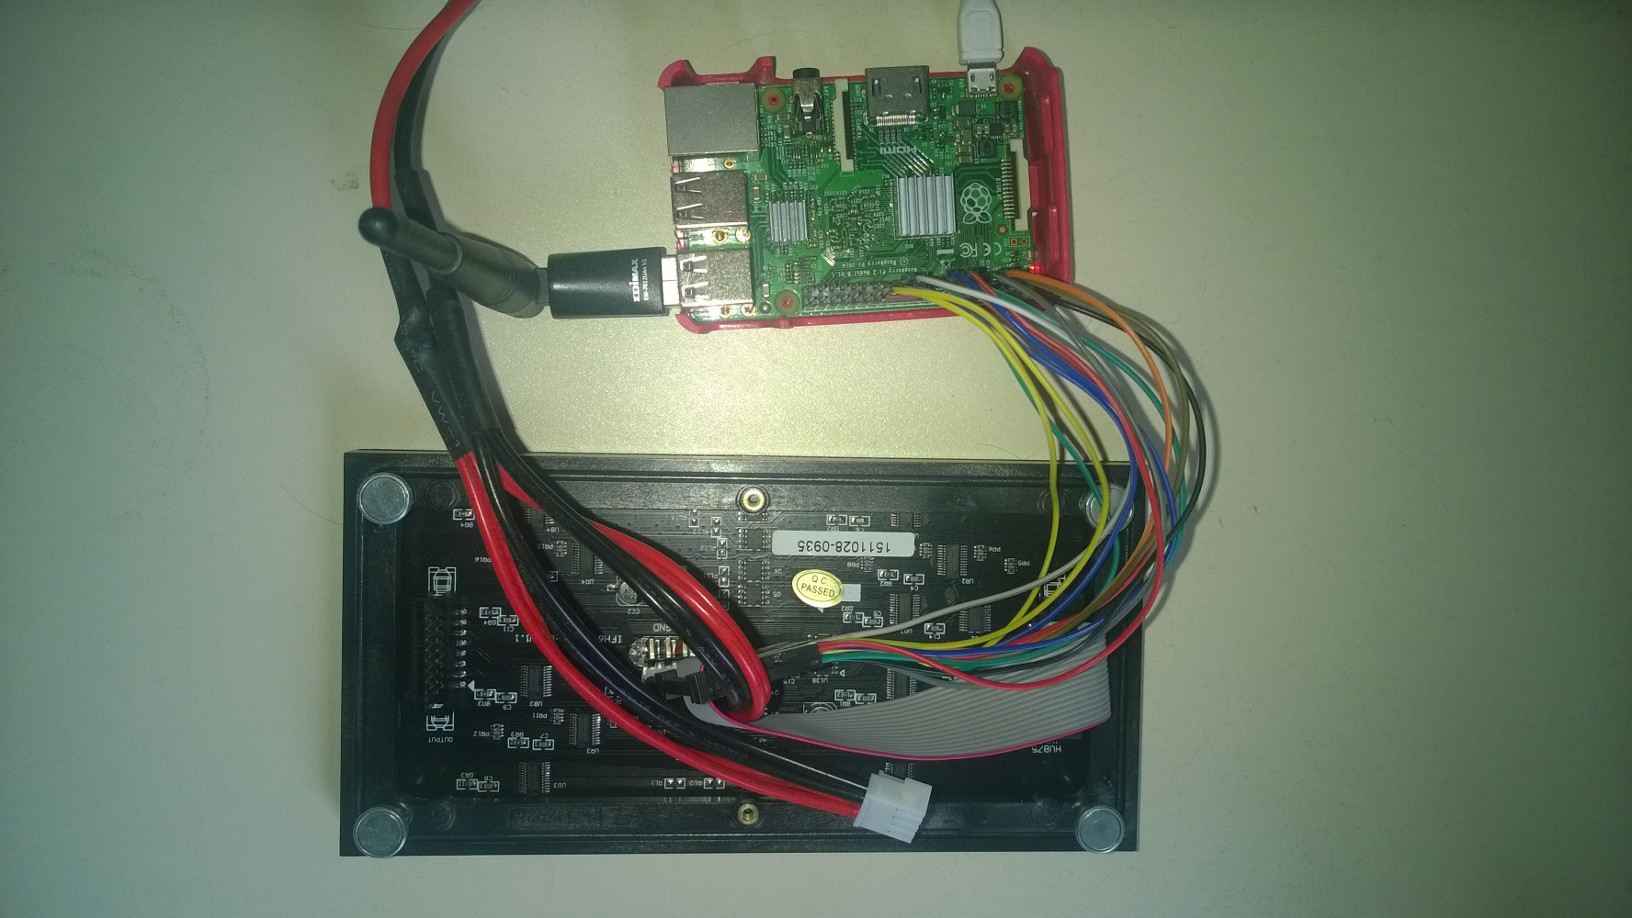
\includegraphics[scale=0.2]{Verkabelung}
	\caption{Verkabelung des Raspberry Pis und der LED-Matrix}
	\label{verkabelung}
\end{figure}

Das Programm wird mit der Programmiersprache Python entwickelt. Um die Signale auf die Pins des Raspberry Pis zu legen, kommt die Bibliothek RPi.GPIO zum Einsatz. Mithilfe der Bibliothek kann eine schnelle Ansteuerung der Pins erfolgen, die Signale können jedoch nur auf 0 oder 1 gelegt werden. Das hat zur Folge, dass die darzustellenden Farben deutlich eingeschränkt sind. Unter Angabe der Pinpositionen werden binäre Signale auf die Pins gelegt und die Matrix angesteuert.

\section{Umsetzung der 4 Gewinnt Logik}
Wie die Ansteuerung der Matrix erfolgt die Implementierung in Python. Eine Klasse \textit{FourWins} dient zur Beschreibung des Spiels, stellt die Rahmenbedingungen fest und steuert den Spielverlauf. Innerhalb dieser Klasse wird sichergestellt, dass Spieler nacheinander ihre Züge machen, der Ablauf eines Zuges definiert und geprüft und ob das Spiel beendet wurde. \textit{FourWins} verfügt über eine 2-dimensionale Liste, welche das aktuelle Spielbrett darstellt. Die Einträge in der Liste stellen dabei den Spieler als kodierte Spielerfarbe dar. Sobald ein Spieler gewinnt werden die 4 gewinnenden Steine in grün eingetragen, um sie hervorzuheben

Das Spiel selbst wird durch die main-Funktion gesteuert. in der main-Funktion werden alternierend Spieler und Eingaben bestimmt, bis das Spiel beendet ist. Um die zu setzende Spalte für den Spieler zu bestimmen wird ein temporärer Index genutzt. Dieser gibt an, in welche Spalte der Stein hineingeworfen wird. Die Spalte kann hierbei durch das drücken der linken bzw. rechten Pfeiltaste ausgewählt werden. Umgesetzt wird dies in Python, indem die Tastatreingaben abgefangen und ausgewertet werden. Die zu setzende Spalte kann schließlich mit der Eingabe-Taste bestätigt werden. Weiter kann das Spiel jederzeit mit Betätigen der \glqq r \grqq -Taste zurückgesetzt und \glqq q \grqq -Taste beendet werden

Die Ansteuerung der LED-Matrix erfolgt in einer eigenen Klasse \textit{LED-Matrix}. Mit Hilfe dieser können je nach Verkabelung die GPIO-Pins ausgewählt werden, die für die Ansteuerung benötigt werden. Desweiteren wird hier das Design des Spielfeldes festgelegt, wie es in Kapitel \ref{sec:ledm} festgelegt wurde.
Die Informationen der Farben für die LED-Matrix werden hierbei innerhalb einer eigenen Liste gespeichert.
Mit Hilfe eines eigenen Threads wird dann mit einer hohen Frequenz das Spielfeld auf der Matrix abgebildet. Durch die fehlende Echtzeitfähigkeit des Raspberry Pis kommt es hierbei allerdings zu einem leicht sichtbaren Flimmern. 
Der blinkende Stein, der zur Darstellung der aktuellen Spalte benötigt wird, wird durch einen internen Timer stets zunächst in der entsprechenden Spielerfarbe angezeigt und wieder ausgeblendet.

\section{Künstliche Intelligenz}
Nachdem die Ansteuerung der Matrix mit Hilfe eines Python Skripts funktioniert, wurde noch eine Kümnstliche Intelligenz (KI) entwickelt, die anhand der gegebenen Informationen und Ressourcen in annehmbarer Zeit eine Zugentscheidung zu produzieren.
Wie in dem Kapitel \ref{sec:vierg} beschrieben handelt es sich bei \glqq Vier Gewinnt\grqq ~um ein Spiel mit perfekter Information handelt. Zusätzlich gehört das Spiel in die Kategorie der Nullsummenspiele. Dies bedeutet, dass die Gewinne und Verluste der beiden Spieler addiert stets 0 ergeben müssen.
Auf Grundlage dieser Informationen ist es möglich für eine KI den Minimax-Algorithmus einzusetzen.

Bei dem Minimax-Algorithmus handelt es sich um einen Gewinnoptimierungsalgorithmus, der über Heuristiken verschiedene Spielsituationen auswertet und den jeweilig besten Zug auswählt.
Für \glqq Vier Gewinnt\grqq ~muss der Algorithmus abgewandelt werden, da der Minimax-Algorithmus in seinen Grundzügen darauf optimiert ist einen maximierenden und einen minimierenden Spieler zu analysieren. Da bei \glqq Vier Gewinnt\grqq ~allerdings beide Spieler maximieren, muss bei der Analyse jeweils darauf geachtet werden, dass das Ergebnis des letzten Spielers negiert wird. Diese Abwandlung wird auch Negamax-Algorithmus genannt.

\begin{algorithm}
\floatname{algorithm}{Algorithmus}
\caption{Negamax-Algorithmus} \label{algo:negamax}
\begin{algorithmic}[1]
\Procedure{NegaMax}{player, depth}
\If {$ depth == 0$~\textbf{or}~$\textit{noPlayableTurns}$} 
\State \Return $\textit{score(player)}$
\EndIf
\State $\textit{maxValue} \gets -\textit{infinity}$
\State $\textit{getPlayableTurns()}$
\While {$\textit{movableTurnsLeft}$}
\State $\textit{makeTurn()}$
\State $\textit{value} \gets -\textit{NegaMax(otherPlayer, depth-1)}$
\State $\textit{redoTurn()}$
\If {$\textit{value} \textgreater \textit{maxValue}$}
\State $\textit{maxValue} \gets \textit{value}$
\If {$\textit{depth} = \textit{requiredDepth}$}
\State $\textit{savedTurn} \gets \textit{turn}$
\EndIf
\EndIf
\EndWhile
\State \Return $\textit{maxValue}$
\EndProcedure
\end{algorithmic}
\end{algorithm}

In Algorithmus \ref{algo:negamax} wird der verwendete Algorithmus als Pseudocode dargestellt.
Auf Grund der begrenzten Rechenkapazitäten, die der Raspberry Pi besitzt, und der hohe Rechenaufwand, der bei einer großen Suchtiefe entsteht, wurde sich dafür entschieden, die Suchtiefe im Rahmen des Projektes auf 4 zu begrenzen. Dabei benötigt der Raspberry Pi immer noch etwa 3 Sekunden, um die Berechnung des Zuges durchzuführen, allerdings liegt diese Zeit in einem akzeptablen Bereich. Da bei dieser Suchtiefe vor allen in den ersten Zügen die Bewertung der einzelnen Spielfeldsituationen teilweise identisch ist, wurde für diesen Fall ein Zufallsmechanismus implementiert, der verhindert, dass die KI deterministisch auszutricksen ist. Insgesamt spielt die KI unter diesen Umständen nicht fehlerfrei, allerdings stellt sie für vor allem ungeübte Spieler eine geeignete Herausforderung da.

	
	% ---------------------------
	% Quellenverzeichnis
	% ---------------------------
	\pagenumbering{Roman}						% Römische Nummerierung
	\setcounter{page}{8} 						% Fortsetzen der Nummerierung

	\printbibliography 								% BiBLaTeX, Biber
	
	% ---------------------------
	% Anhang
	% ---------------------------
	\appendix
	\include{include/anhang}
	
\end{document}
